\documentclass[border=12pt]{standalone}
\usepackage{tikz}
\usetikzlibrary{positioning, calc, fit, backgrounds, arrows.meta}
\usepackage{amsmath, amssymb}

\begin{document}
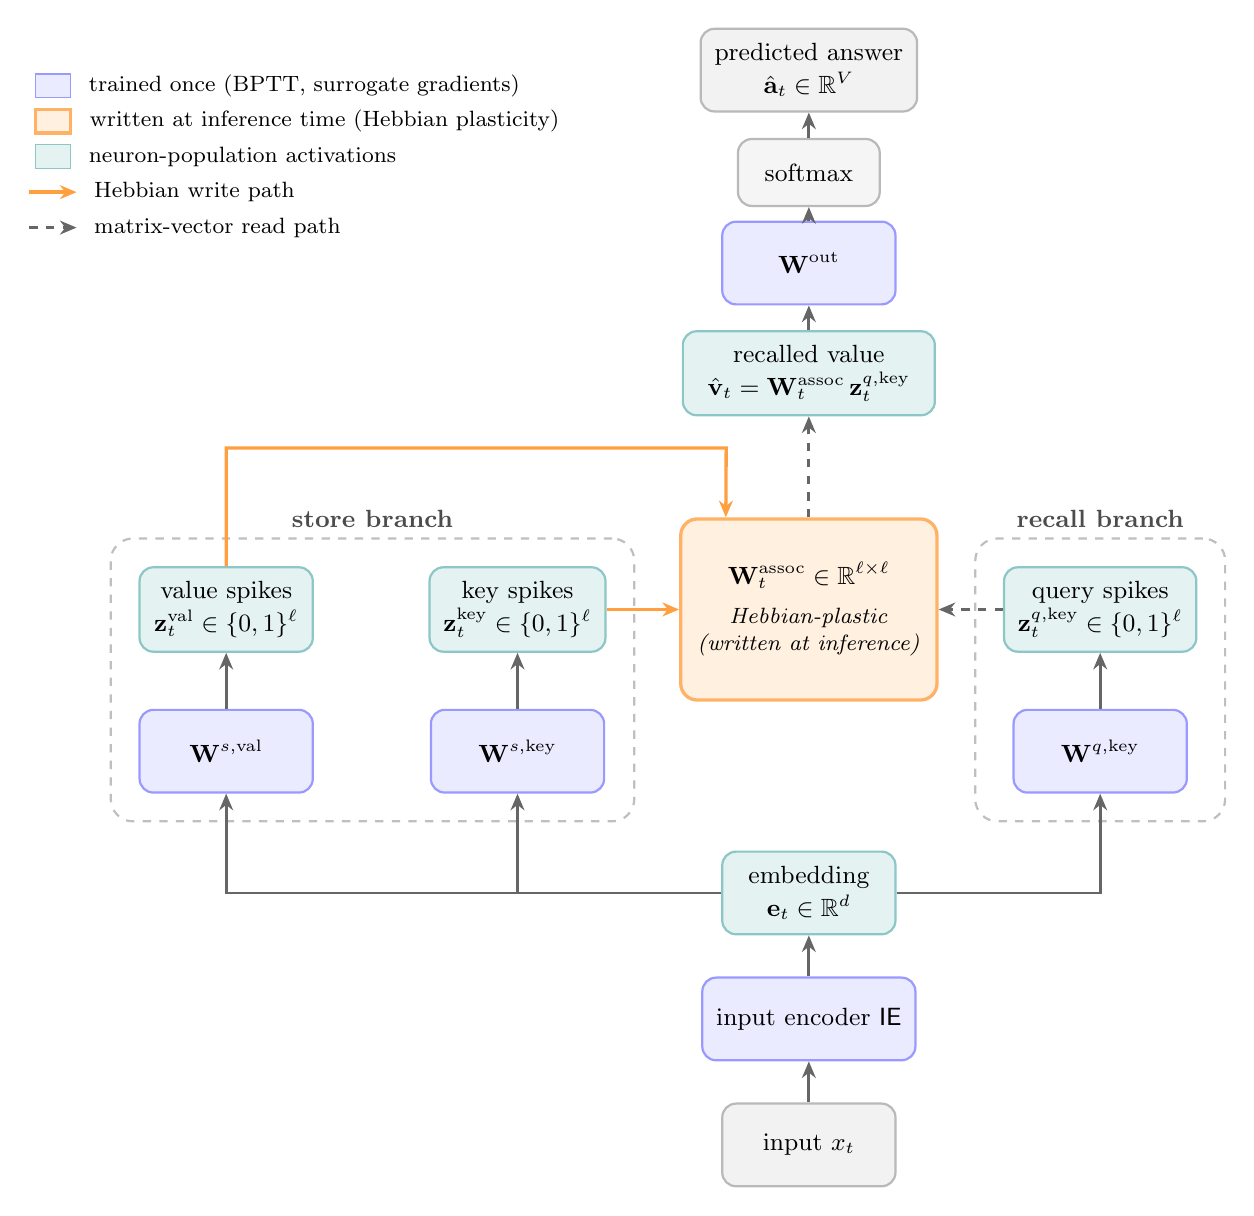
\begin{tikzpicture}[
    mainblock/.style  = {rectangle, draw=gray!55, thick, rounded corners=5pt,
                         minimum height=1.05cm, minimum width=2.20cm,
                         font=\small, inner sep=5pt, align=center},
    trnblock/.style   = {mainblock, fill=blue!8,    draw=blue!40},
    actblock/.style   = {mainblock, fill=teal!10,   draw=teal!45},
    hebblock/.style   = {rectangle, draw=orange!60, very thick, rounded corners=6pt,
                         minimum height=2.30cm, minimum width=3.20cm,
                         font=\small, inner sep=6pt, align=center,
                         fill=orange!12},
    ioblock/.style    = {mainblock, fill=gray!10,   draw=gray!55},
    softblock/.style  = {mainblock, fill=gray!8,    draw=gray!55,
                         minimum width=1.80cm, minimum height=0.85cm},
    conn/.style       = {line width=1.0pt, draw=black!60,
                         -{Stealth[length=6pt, width=5pt]}},
    plastconn/.style  = {line width=1.2pt, draw=orange!75,
                         -{Stealth[length=6pt, width=5pt]}},
    readconn/.style   = {line width=1.0pt, draw=black!60, dashed,
                         -{Stealth[length=6pt, width=5pt]}},
    annot/.style      = {font=\footnotesize, text=black!55, align=center},
    branchlbl/.style  = {font=\small\bfseries, text=black!70, align=center},
    titlelbl/.style   = {font=\small\bfseries, text=black!80, align=center},
    legendboxA/.style = {rectangle, draw=blue!40, fill=blue!8,
                         minimum width=0.45cm, minimum height=0.30cm, inner sep=0pt},
    legendboxB/.style = {rectangle, draw=orange!60, fill=orange!12, very thick,
                         minimum width=0.45cm, minimum height=0.30cm, inner sep=0pt},
    legendboxC/.style = {rectangle, draw=teal!45, fill=teal!10,
                         minimum width=0.45cm, minimum height=0.30cm, inner sep=0pt},
    branchbox/.style  = {rectangle, draw=black!25, dashed, thick,
                         rounded corners=8pt, inner sep=10pt},
    valboxwide/.style = {mainblock, fill=teal!10, draw=teal!45,
                         minimum width=3.00cm},
    readoutwide/.style= {mainblock, fill=teal!10, draw=teal!45,
                         minimum width=3.20cm},
]

%% ============================================================
%% LAYOUT — symmetric heights, recalled-value box matches memory width.
%% Value-write arrow rises FROM value-spikes upward, then travels right
%% along a dedicated lane ABOVE the branch boxes, then drops into the
%% top of the memory. This avoids any block-crossings.
%% ============================================================
\def\xStoreV{-7.4}
\def\xStoreK{-3.7}
\def\xMem{0.0}
\def\xRecallK{3.7}
\def\xMid{0.0}

\def\yIn{-5.4}
\def\yEnc{-3.8}
\def\yEmbed{-2.2}
\def\yProj{-0.4}
\def\yKV{1.4}        % both value-spikes and key-spikes at this height
\def\yMem{1.4}
\def\yWriteLane{3.45} % above branch boxes; value-write travels along here
\def\yReadout{4.4}
\def\yWout{5.8}
\def\ySoft{6.95}
\def\yOut{8.25}

%% ============================================================
%% INPUT and ENCODER (bottom)
%% ============================================================
\node[ioblock]  (xt)   at (\xMid, \yIn)   {input $x_{t}$};
\node[trnblock] (IE)   at (\xMid, \yEnc)  {input encoder \textsf{IE}};
\node[actblock] (et)   at (\xMid, \yEmbed){embedding\\[1pt]$\mathbf{e}_{t}\in\mathbb{R}^{d}$};
\draw[conn] (xt.north) -- (IE.south);
\draw[conn] (IE.north) -- (et.south);

%% ============================================================
%% STORE BRANCH (left)
%% ============================================================
\node[trnblock] (Wsv)  at (\xStoreV, \yProj) {$\mathbf{W}^{s,\text{val}}$};
\node[trnblock] (Wsk)  at (\xStoreK, \yProj) {$\mathbf{W}^{s,\text{key}}$};
\node[actblock] (vs)   at (\xStoreV, \yKV)
    {value spikes\\[1pt]$\mathbf{z}^{\text{val}}_{t}\in\{0,1\}^{\ell}$};
\node[actblock] (ks)   at (\xStoreK, \yKV)
    {key spikes\\[1pt]$\mathbf{z}^{\text{key}}_{t}\in\{0,1\}^{\ell}$};

\draw[conn] (et.west) -| (Wsv.south);
\draw[conn] (et.west) -| (Wsk.south);
\draw[conn] (Wsv.north) -- (vs.south);
\draw[conn] (Wsk.north) -- (ks.south);

%% ============================================================
%% RECALL BRANCH (right)
%% ============================================================
\node[trnblock] (Wqk)  at (\xRecallK, \yProj) {$\mathbf{W}^{q,\text{key}}$};
\node[actblock] (kq)   at (\xRecallK, \yKV)
    {query spikes\\[1pt]$\mathbf{z}^{q,\text{key}}_{t}\in\{0,1\}^{\ell}$};
\draw[conn] (et.east) -| (Wqk.south);
\draw[conn] (Wqk.north) -- (kq.south);

%% ============================================================
%% MEMORY (center)
%% ============================================================
\node[hebblock] (Wmem) at (\xMem, \yMem)
    {$\mathbf{W}^{\text{assoc}}_{t}\in\mathbb{R}^{\ell\times\ell}$\\[3pt]
     \footnotesize \textit{Hebbian-plastic}\\[-1pt]
     \footnotesize \textit{(written at inference)}};

%% Write paths:
%%  - key spikes: straight right into the LEFT edge of memory.
%%  - value spikes: up to the dedicated write-lane, right along it,
%%    then DOWN into the TOP-LEFT corner of the memory. No block crossings.
\draw[plastconn] (ks.east) -- (Wmem.west);
\draw[plastconn] (vs.north) |- (\xMem - 1.05, \yWriteLane) -- ([xshift=-30pt]Wmem.north);

%% Read input: query spikes -> right edge of memory
\draw[readconn] (kq.west) -- (Wmem.east);

%% Recalled value: same width as the memory, sitting directly above it.
\node[readoutwide] (vread) at (\xMid, \yReadout)
    {recalled value\\[1pt]$\hat{\mathbf{v}}_{t} = \mathbf{W}^{\text{assoc}}_{t}\,\mathbf{z}^{q,\text{key}}_{t}$};
\draw[readconn] (Wmem.north) -- (vread.south);

%% ============================================================
%% READOUT STACK
%% ============================================================
\node[trnblock]  (Wout)   at (\xMid, \yWout) {$\mathbf{W}^{\text{out}}$};
\node[softblock] (soft)   at (\xMid, \ySoft) {softmax};
\node[ioblock]   (ahat)   at (\xMid, \yOut)
    {predicted answer\\[1pt]$\hat{\mathbf{a}}_{t}\in\mathbb{R}^{V}$};

\draw[conn] (vread.north) -- (Wout.south);
\draw[conn] (Wout.north)  -- (soft.south);
\draw[conn] (soft.north)  -- (ahat.south);

%% ============================================================
%% BRANCH GROUPING
%% ============================================================
\begin{pgfonlayer}{background}
\node[branchbox, fit=(Wsv) (Wsk) (vs) (ks)] (storeBox) {};
\node[branchbox, fit=(Wqk) (kq)] (recallBox) {};
\end{pgfonlayer}

\node[branchlbl, anchor=south] at (storeBox.north)  {store branch};
\node[branchlbl, anchor=south] at (recallBox.north) {recall branch};

%% ============================================================
%% LEGEND (top-left)
%% ============================================================
\def\xLeg{-9.6}
\def\yLeg{\yOut - 0.2}
\node[legendboxA] (legA) at (\xLeg, \yLeg) {};
\node[anchor=west, font=\footnotesize] at ($(legA.east) + (0.10,0)$)
    {trained once (BPTT, surrogate gradients)};

\node[legendboxB] (legB) at (\xLeg, \yLeg - 0.45) {};
\node[anchor=west, font=\footnotesize] at ($(legB.east) + (0.10,0)$)
    {written at inference time (Hebbian plasticity)};

\node[legendboxC] (legC) at (\xLeg, \yLeg - 0.90) {};
\node[anchor=west, font=\footnotesize] at ($(legC.east) + (0.10,0)$)
    {neuron-population activations};

\draw[plastconn] ($(\xLeg - 0.30, \yLeg - 1.35)$) -- ($(\xLeg + 0.30, \yLeg - 1.35)$);
\node[anchor=west, font=\footnotesize] at ($(\xLeg + 0.40, \yLeg - 1.35)$)
    {Hebbian write path};

\draw[readconn] ($(\xLeg - 0.30, \yLeg - 1.80)$) -- ($(\xLeg + 0.30, \yLeg - 1.80)$);
\node[anchor=west, font=\footnotesize] at ($(\xLeg + 0.40, \yLeg - 1.80)$)
    {matrix-vector read path};

\end{tikzpicture}
\end{document}
